\subsection{Video-Produktion}
Ein Trailer zu unserem Produkt (Videospiel), sollte erstellt werden. Dieses ca. 1 Minute Video soll im BB-Gebäude in einer Dauerschleife mit den anderen interdisziplinären Projekten aus unserem Studiengang an großen Monitoren gezeigt werden. Der Trailer soll einen kurzen Einblick zu unserem Videospiel geben. Dabei soll die Tonalität und Spezifizierung unseres Produkts (Cardgame) schnell erkennbar sein. Nach einer Ideensammlung einiger Teammitglieder in Form von Storyboards, wurde sich auf einen groben Aufbau geeinigt.
Um einen gewissen Überblick über den dramaturgischen Ablauf zu kriegen, hat Robert Sabo ein Videoscript zum Trailer angefertigt(Siehe Datei: Video-Teaser-Trailer/Videoscript.pdf). In diesem Script steht allgemein der Zeichenstil, die Schriftarten, Länge der Abschnitte und deren Einstellungen, sowie allgemeine Schnittkonventionen. Die Handlung wurde in mehrere Einstellungen aufgeteilt, die eine gewisse Dramaturgie unterstützen. Visuelle und auditive Angaben wurden hier auch festgelegt. Die jeweils drei Abschnitte wurden unter den Beteiligten aufgeteilt (Abschnitt 1: Manuela, Abschnitt 2: Robert, Abschnitt 3: Gabriel). Sämtliche Videosegmente wurden mit Adobe After Effekts realisiert. Die einzelnen Assets wurden mit Adobe Photoshop erstellt. Schlussendlich wurden die drei Abschnitte von allen Beteiligenten von Robert Sabo einheitlich in After Effekts zusammengeschnitten. Dabei war es wichtig die Tonalität gut herüberzubringen. Deshalb mussten Paar Abschnitte neu bzw. angepasst werden, um einheitlich zu wirken. Schlussendlich wurde die Datei im avi-Format gerendert. Da die Datei aber zu groß war, wurde sie mit Hilfe von Pia Korndörfer zu einem kleineren Format, mp4, komprimiert. Philadelphia Gauß hat noch extra für die Präsentation eine Trailer-Version mit Soundeffekten und Soundtrack erstellt, um auch einen passenden auditiven Eindruck des Videospiels für die Zuschauer zu geben.

Auf die einzelnen Abschnitte wird im Folgenden genauer eingegangen.

\subsubsection{Einarbeitung in After Effects}
Zunächst einmal erfolgte eine intensive Einarbeitungsphase mit dem Programm „After Effects“. Dabei waren sehr gute Youtube Tutorials eine große Unterstützung. 
Das Resultat von dem ersten Testvideo schaut wie folgt aus: 
\begin{figure}[h]
\centering
 \subfloat[Screenshot: After Effects 1]{{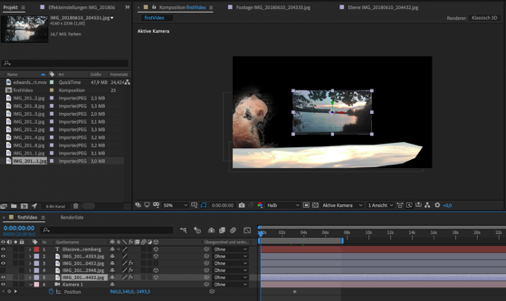
\includegraphics[width=5cm]{../img/screenshot_aftereffects_1.PNG} }}
\qquad
 \subfloat[Screenshot: After Effects 2]{{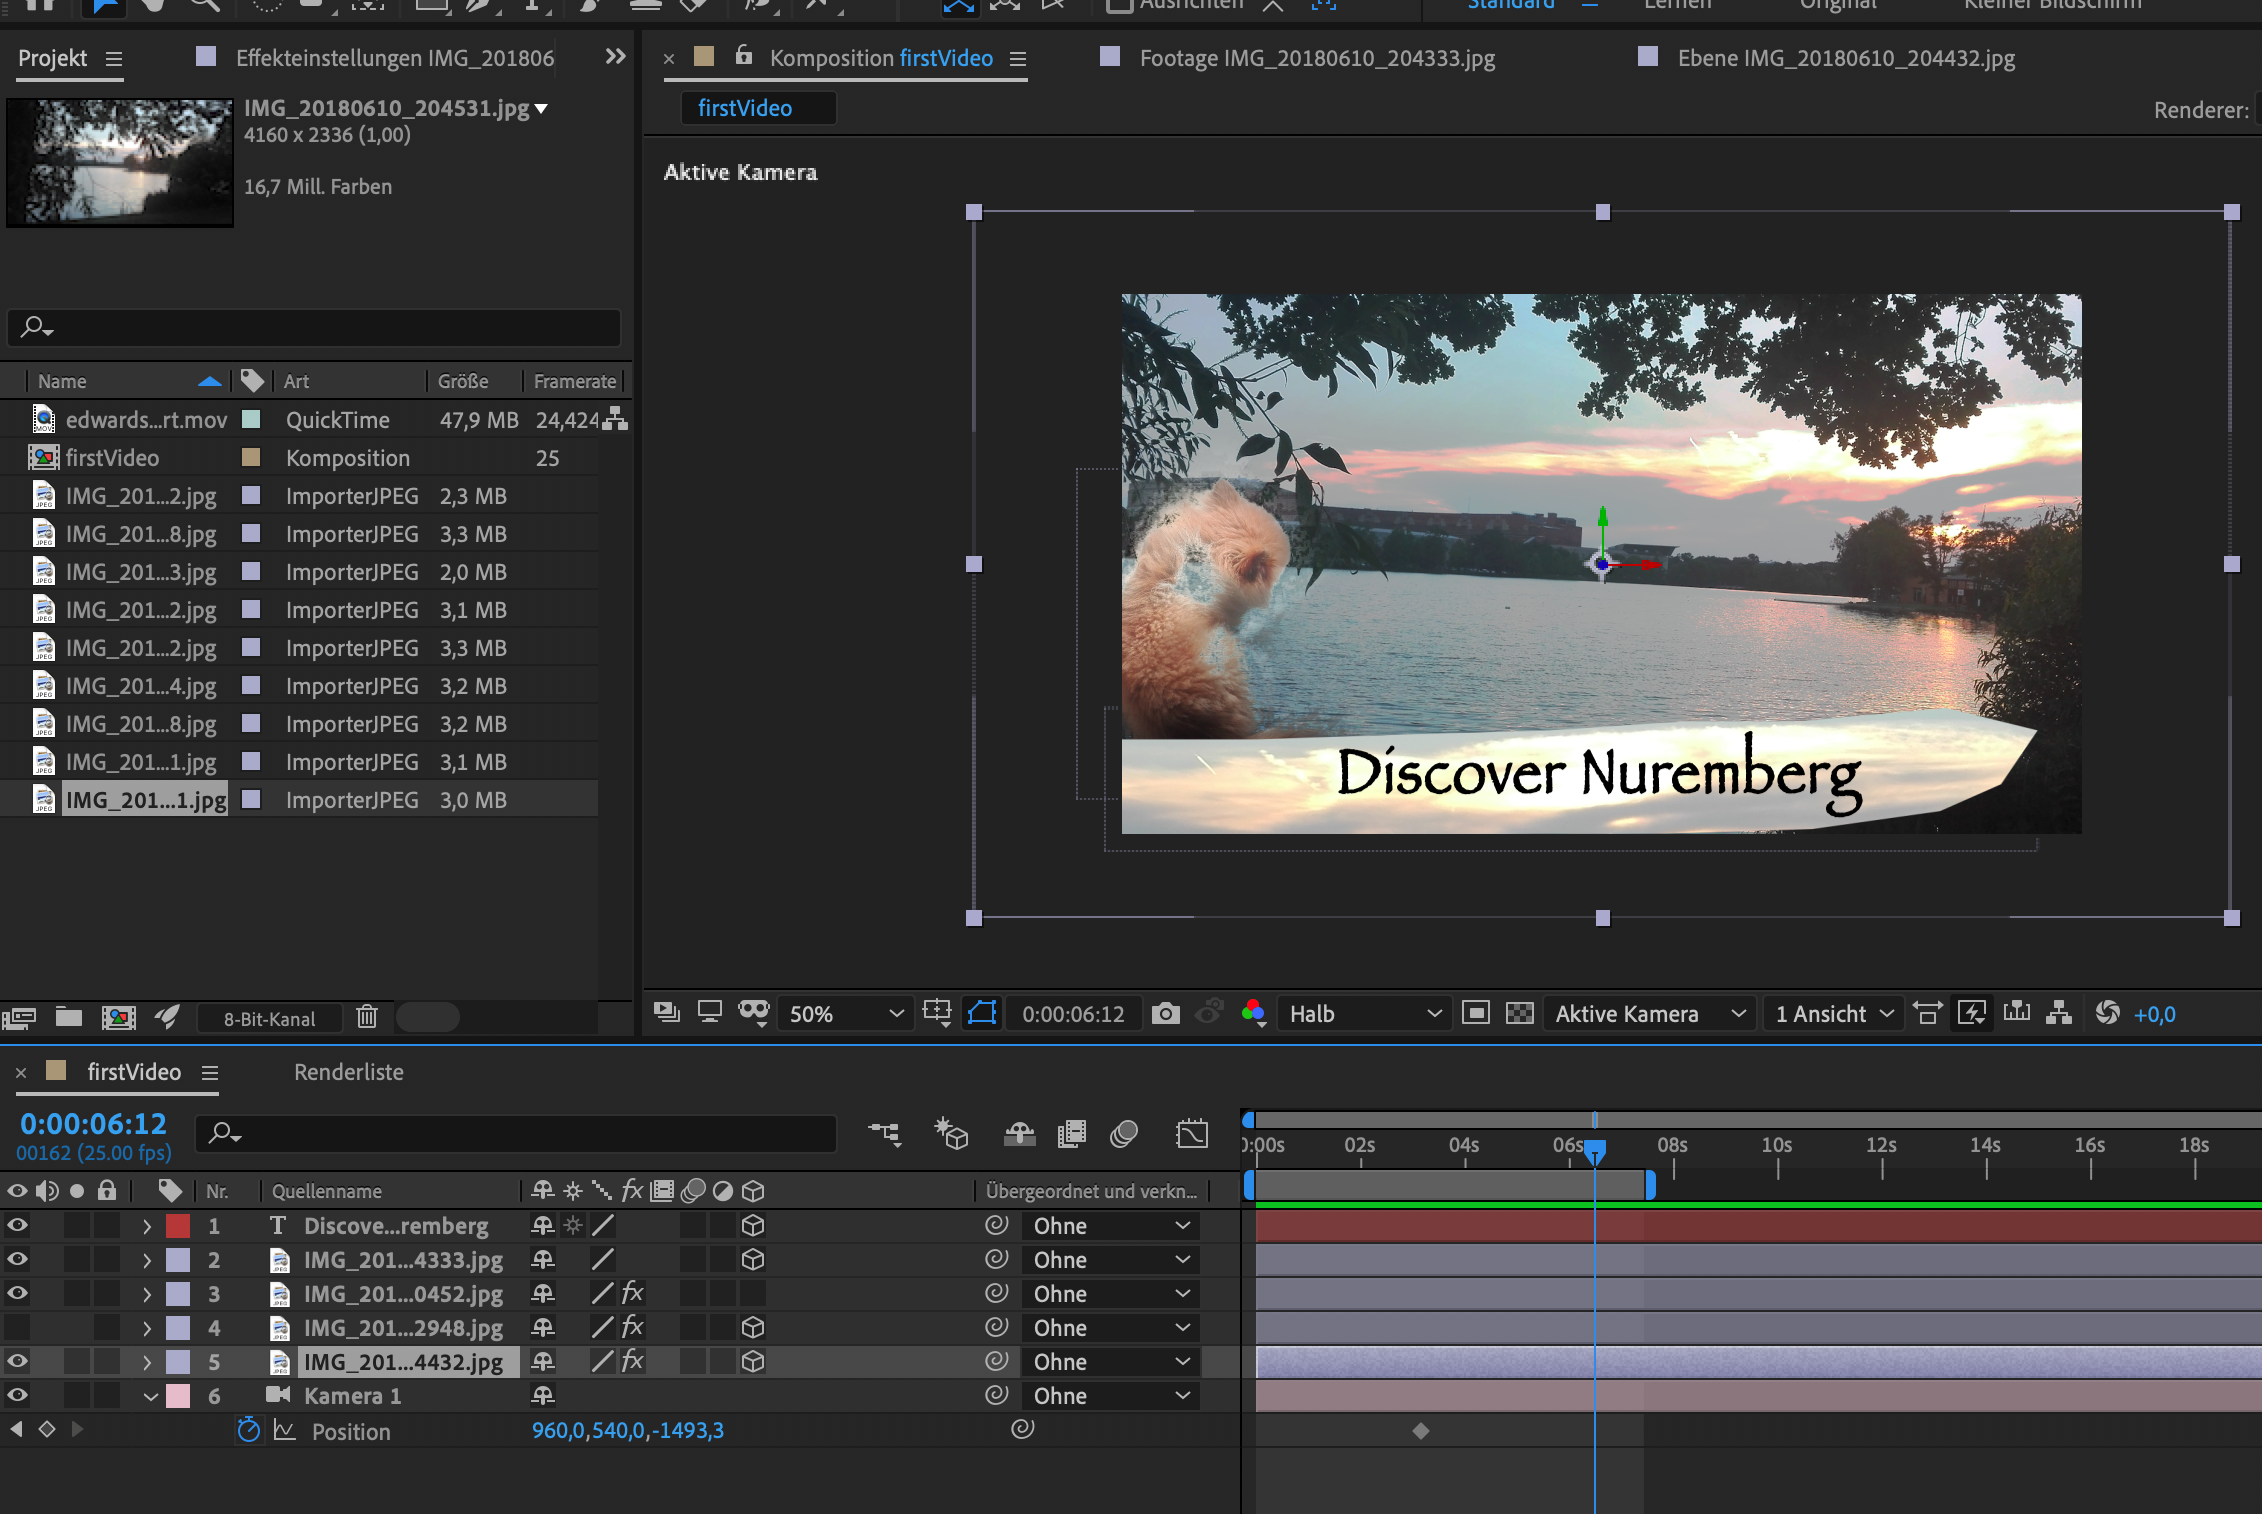
\includegraphics[width=5cm]{../img/screenshot_aftereffects_2.PNG} }}
\caption{Screenshots After Effects}%
 \label{fig:Screenshots After Effect}%
\end{figure}
Hierbei wurden Bilder freigestellt, ein Bild und der Titel animiert.  

\subsubsection{Animation des Logos}
Das Video endet, wie in vielen bekannten Videos, mit unserem Logo. Hierfür musste das Edwards Biotope Logo animiert werden. 
Zunächst einmal wurde die Grafik (links) von dem Text (rechts) separiert. Die Absicht war es, zuerst das Symbol animiert einzublenden. Im Anschluss taucht der Name „Edwards Biotope“ auf. Dieser Text wurde ebenso animiert. Zum Schluss werden beide Teile wieder zusammengefügt. Die Bildreihenfolge Abbildung \ref{fig:Screenshots Animations 1} stellt diese Logo Animation dar. 
\begin{figure}[h]
\centering
 \subfloat[Screenshot: Animation 1]{{
\includegraphics[width=2cm]{../img/logo_animation/1/screenshot_logo_1.PNG} }}
\qquad
 \subfloat[Screenshot: Animation 2]{{
\includegraphics[width=2cm]{../img/logo_animation/1/screenshot_logo_2.PNG} }}
\qquad
 \subfloat[Screenshot: Animation 3]{{
\includegraphics[width=2cm]{../img/logo_animation/1/screenshot_logo_3.PNG} }}
\qquad
 \subfloat[Screenshot: Animation 4]{{
\includegraphics[width=2cm]{../img/logo_animation/1/screenshot_logo_4.PNG} }}
\caption{Screenshots Animations 1}%
 \label{fig:Screenshots Animations 1}%
\end{figure}

Allerdings war das nicht sehr überzeugend. Daher wurde weiterhin experimentiert. So wurde das Logo mit dem Spielnamen nicht mehr separiert animiert, sondern von Anfang an zusammen. Der Bildablauf  Abbildung \ref{fig:Screenshots Animations 2} veranschaulicht diese Animation.

\begin{figure}[h]
\centering
 \subfloat[Screenshot: Animation 5]{{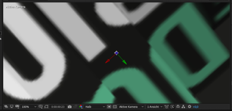
\includegraphics[width=2cm]{../img/logo_animation/2/screenshot_logo_5.PNG} }}
\qquad
 \subfloat[Screenshot: Animation 6]{{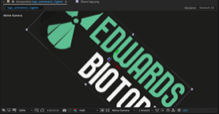
\includegraphics[width=2cm]{../img/logo_animation/2/screenshot_logo_6.PNG} }}
\qquad
 \subfloat[Screenshot: Animation 7]{{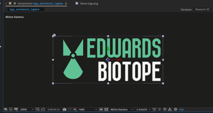
\includegraphics[width=2cm]{../img/logo_animation/2/screenshot_logo_7.PNG} }}
\caption{Screenshots Animations 2}%
 \label{fig:Screenshots Animations 2}%
\end{figure}

Im Anschluss wurde ein CC Light Sweep Effekt hinzugefügt und dafür gesorgt, dass das Logo kurz glänzt. Mit der Bestimmung der Richtung verläuft dieser Effekt von links oben nach rechts unten. Dieser Effekt ist auf der Abbildung \ref{fig:Screenshots Animations 3} zu sehen.

\begin{figure}[h]
\centering
 \subfloat[Screenshot: Animation 8]{{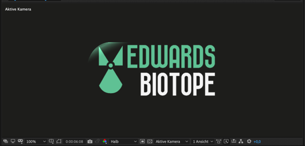
\includegraphics[width=2cm]{../img/logo_animation/3/screenshot_logo_8.PNG} }}
\qquad
 \subfloat[Screenshot: Animation 9]{{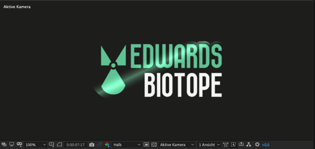
\includegraphics[width=2cm]{../img/logo_animation/3/screenshot_logo_9.PNG} }}
\qquad
 \subfloat[Screenshot: Animation 10]{{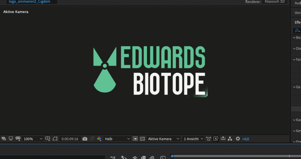
\includegraphics[width=2cm]{../img/logo_animation/3/screenshot_logo_10.PNG} }}
\caption{Screenshots Animations 3}%
 \label{fig:Screenshots Animations 3}%
\end{figure}

\subsubsection{Animation des Logos für denn Trailer}
Für den Trailer fehlte am Ende des Trailers eine Logoanimation. Die Animation wurde mit Adobe After Effects erstellt. Als Material für die Animation wurde das Logo benötigt und ein Hintergrund, der mit der Spielwelt von Edwards Biotope harmoniert. Deshalb wurde als Hintergrund ein Video Clip von Vimeo gesucht, das unter Creative Common Lizenz verwendet werden darf. Es wurde sich für einen Wellengang bei Sonnenuntergang im Meer entschieden. Das Logo wurde passend zu der Wellenbewegung animiert. Mit der letzten Welle wird das Logo unter das Wasser gespült und soll somit das abtauchen in die Unterwasser-Spielwelt von EDWARDS BIOTOPE symbolisieren. Die Logoanimation wurde noch einmal überarbeitet, um alle Einzelteile des Trailers aneinander anzupassen. 
Die Animation befindet sich entsprechend im Anhang unter Logoanimation.

\subsubsection{Kompression des Trailers}
Das Endprodukt des Trailers war eine 8GB unkomprimierte AVI Video-Datei. In dieser Größe konnte es nicht auf den Server der Hochschule hochgeladen werden. Deshalb musste der Trailer noch komprimiert werden. Die Komprimierung erfolgte mit dem Adobe Media Encoder. Als Dateiformat wurde MOV ausgewählt. MOV hat den Vorteil, die Datenmenge mit verlustfreier und verlustbehaftender Komprimierung auf 70 MB zu verringern ohne sichtbare Qualitätsverluste zu liefern.
Die Animation befindet sich entsprechend im Anhang unter Logoanimation.


\subsubsection{Storyboard}
Für die Präsentation des Projekts musste ein kurzer Trailer angefertigt werden, der unser Projekt innerhalb einer Minute grob darstellt und dem Zuschauer Lust auf unser Spiel macht. Um erste Anregungen zu sammeln, wurde sich zusammengesetzt und Ideen miteinander ausgetauscht. Im Anschluss bekamen Gabriel, Pamela, Cigdem und Manuela die Aufgabe, Storyboards anzufertigen. Somit sollten die gesammelten Ideen veranschaulicht werden.
Ein Storyboard ist eine Art visuelles Drehbuch, in dem Abläufe von Szenen konzipiert werden. Es kann skizziert, aber auch collagiert sein. Innerhalb des Storyboards können Kameraschnitte, Bewegungsanweisungen, Überblendungen und auditive Ansagen festgehalten werden.
Der Trailer muss den Zuschauer in die Unterwasserwelt von EDWARDS BIOTOPE eintauchen lassen und sowohl einen Vorgeschmack für die Hintergrundgeschichte als auch eine kurze Sicht auf die Spielmechanik bieten. Dennoch sollte eine Länge von einer Minute nicht überschritten werden. Genau das galt es bei der Erstellung der Storyboards zu beachten. Das entsprechende Storyboard ist im Anhang beigefügt. 

Letztendlich wurde sich nicht für eines der Storyboards entschieden, sondern es wurden die verschiedenen Umsetzungen miteinander kombiniert. Dies ergab schließlich die Vorgabe für unseren Trailer, der dann von Robert und Pia umgesetzt wurde.

In unserem Gameplay-Trailer sollte der grobe Spielablauf dargestellt werden. Als Programm wurde Adobe After Effects CC verwendet.
Wie bereits Eingangs beschrieben, wurden für das Video mehrere Storyboards angefertigt. Hierzu ein Auszug in Abbildung \ref{Storyboard: Spielfeld}

\begin{figure}[h]
\centering
 \subfloat[Storyboard: Spielfeld 1]{{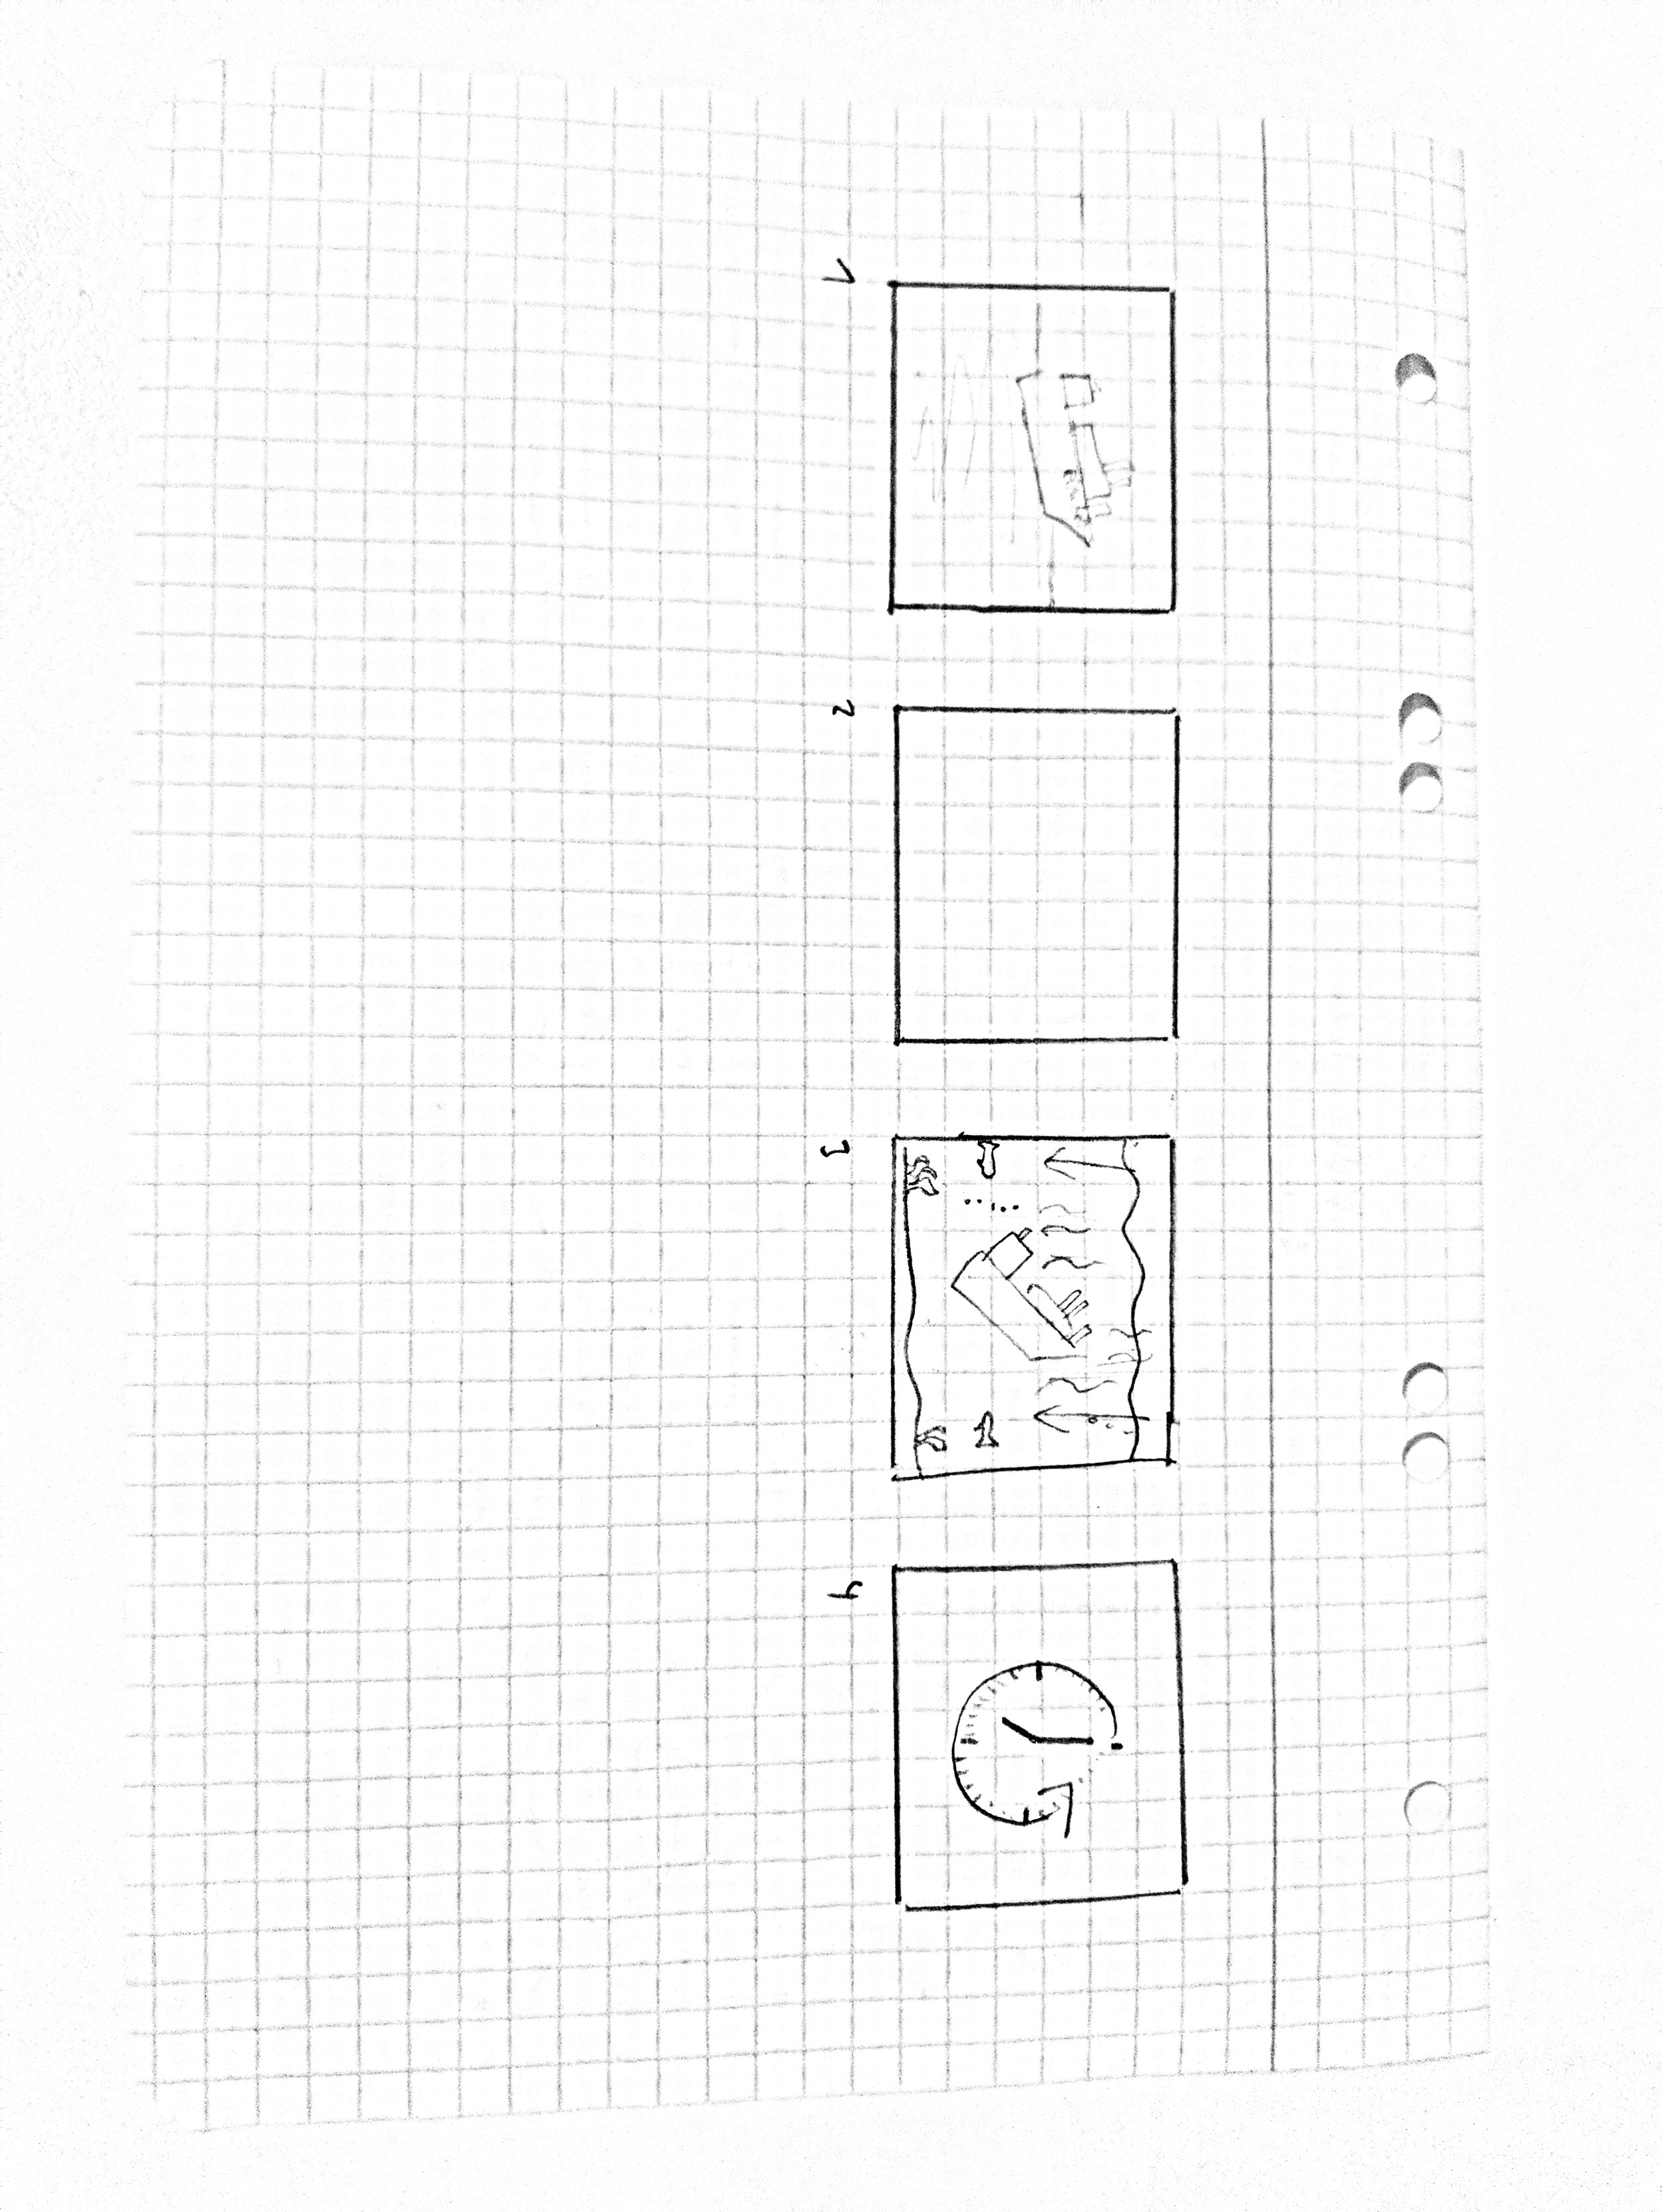
\includegraphics[width=4cm]{../img/storyboards/storyboard_1.JPG} }}
\qquad
 \subfloat[Storyboard: Spielfeld 2]{{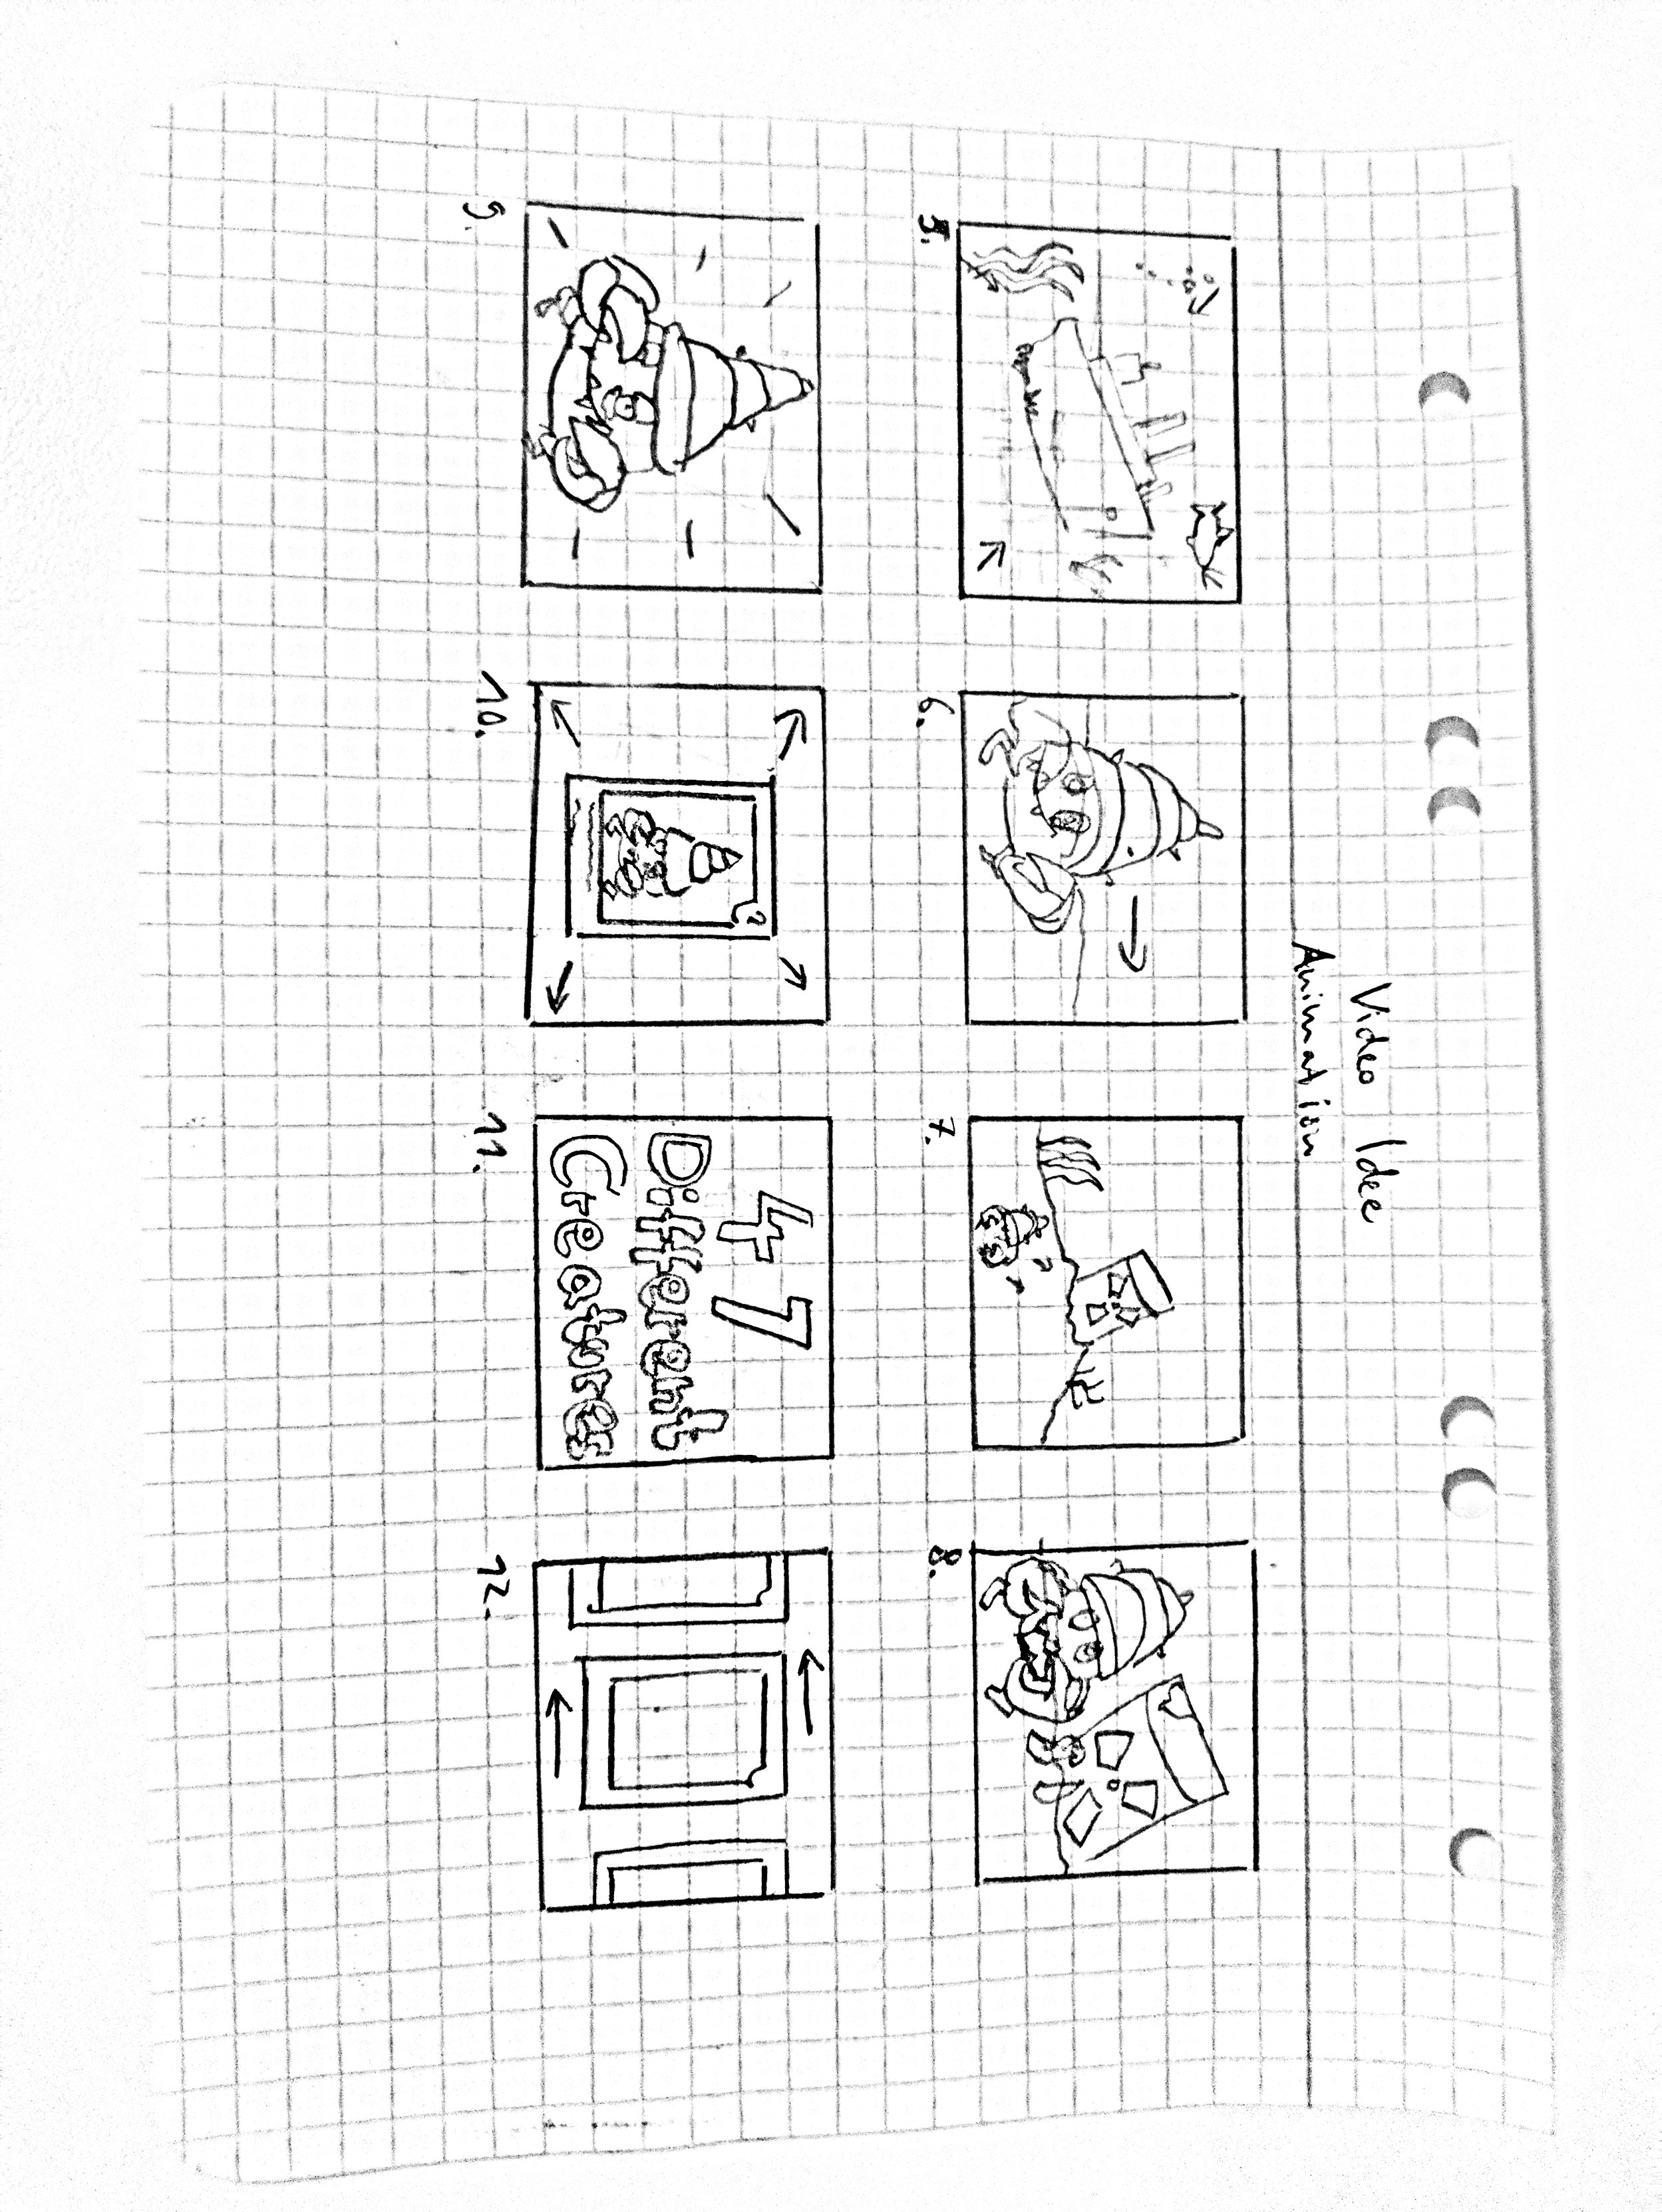
\includegraphics[width=4cm]{../img/storyboards/storyboard_2.JPG} }}
\qquad
 \subfloat[Storyboard: Spielfeld 3]{{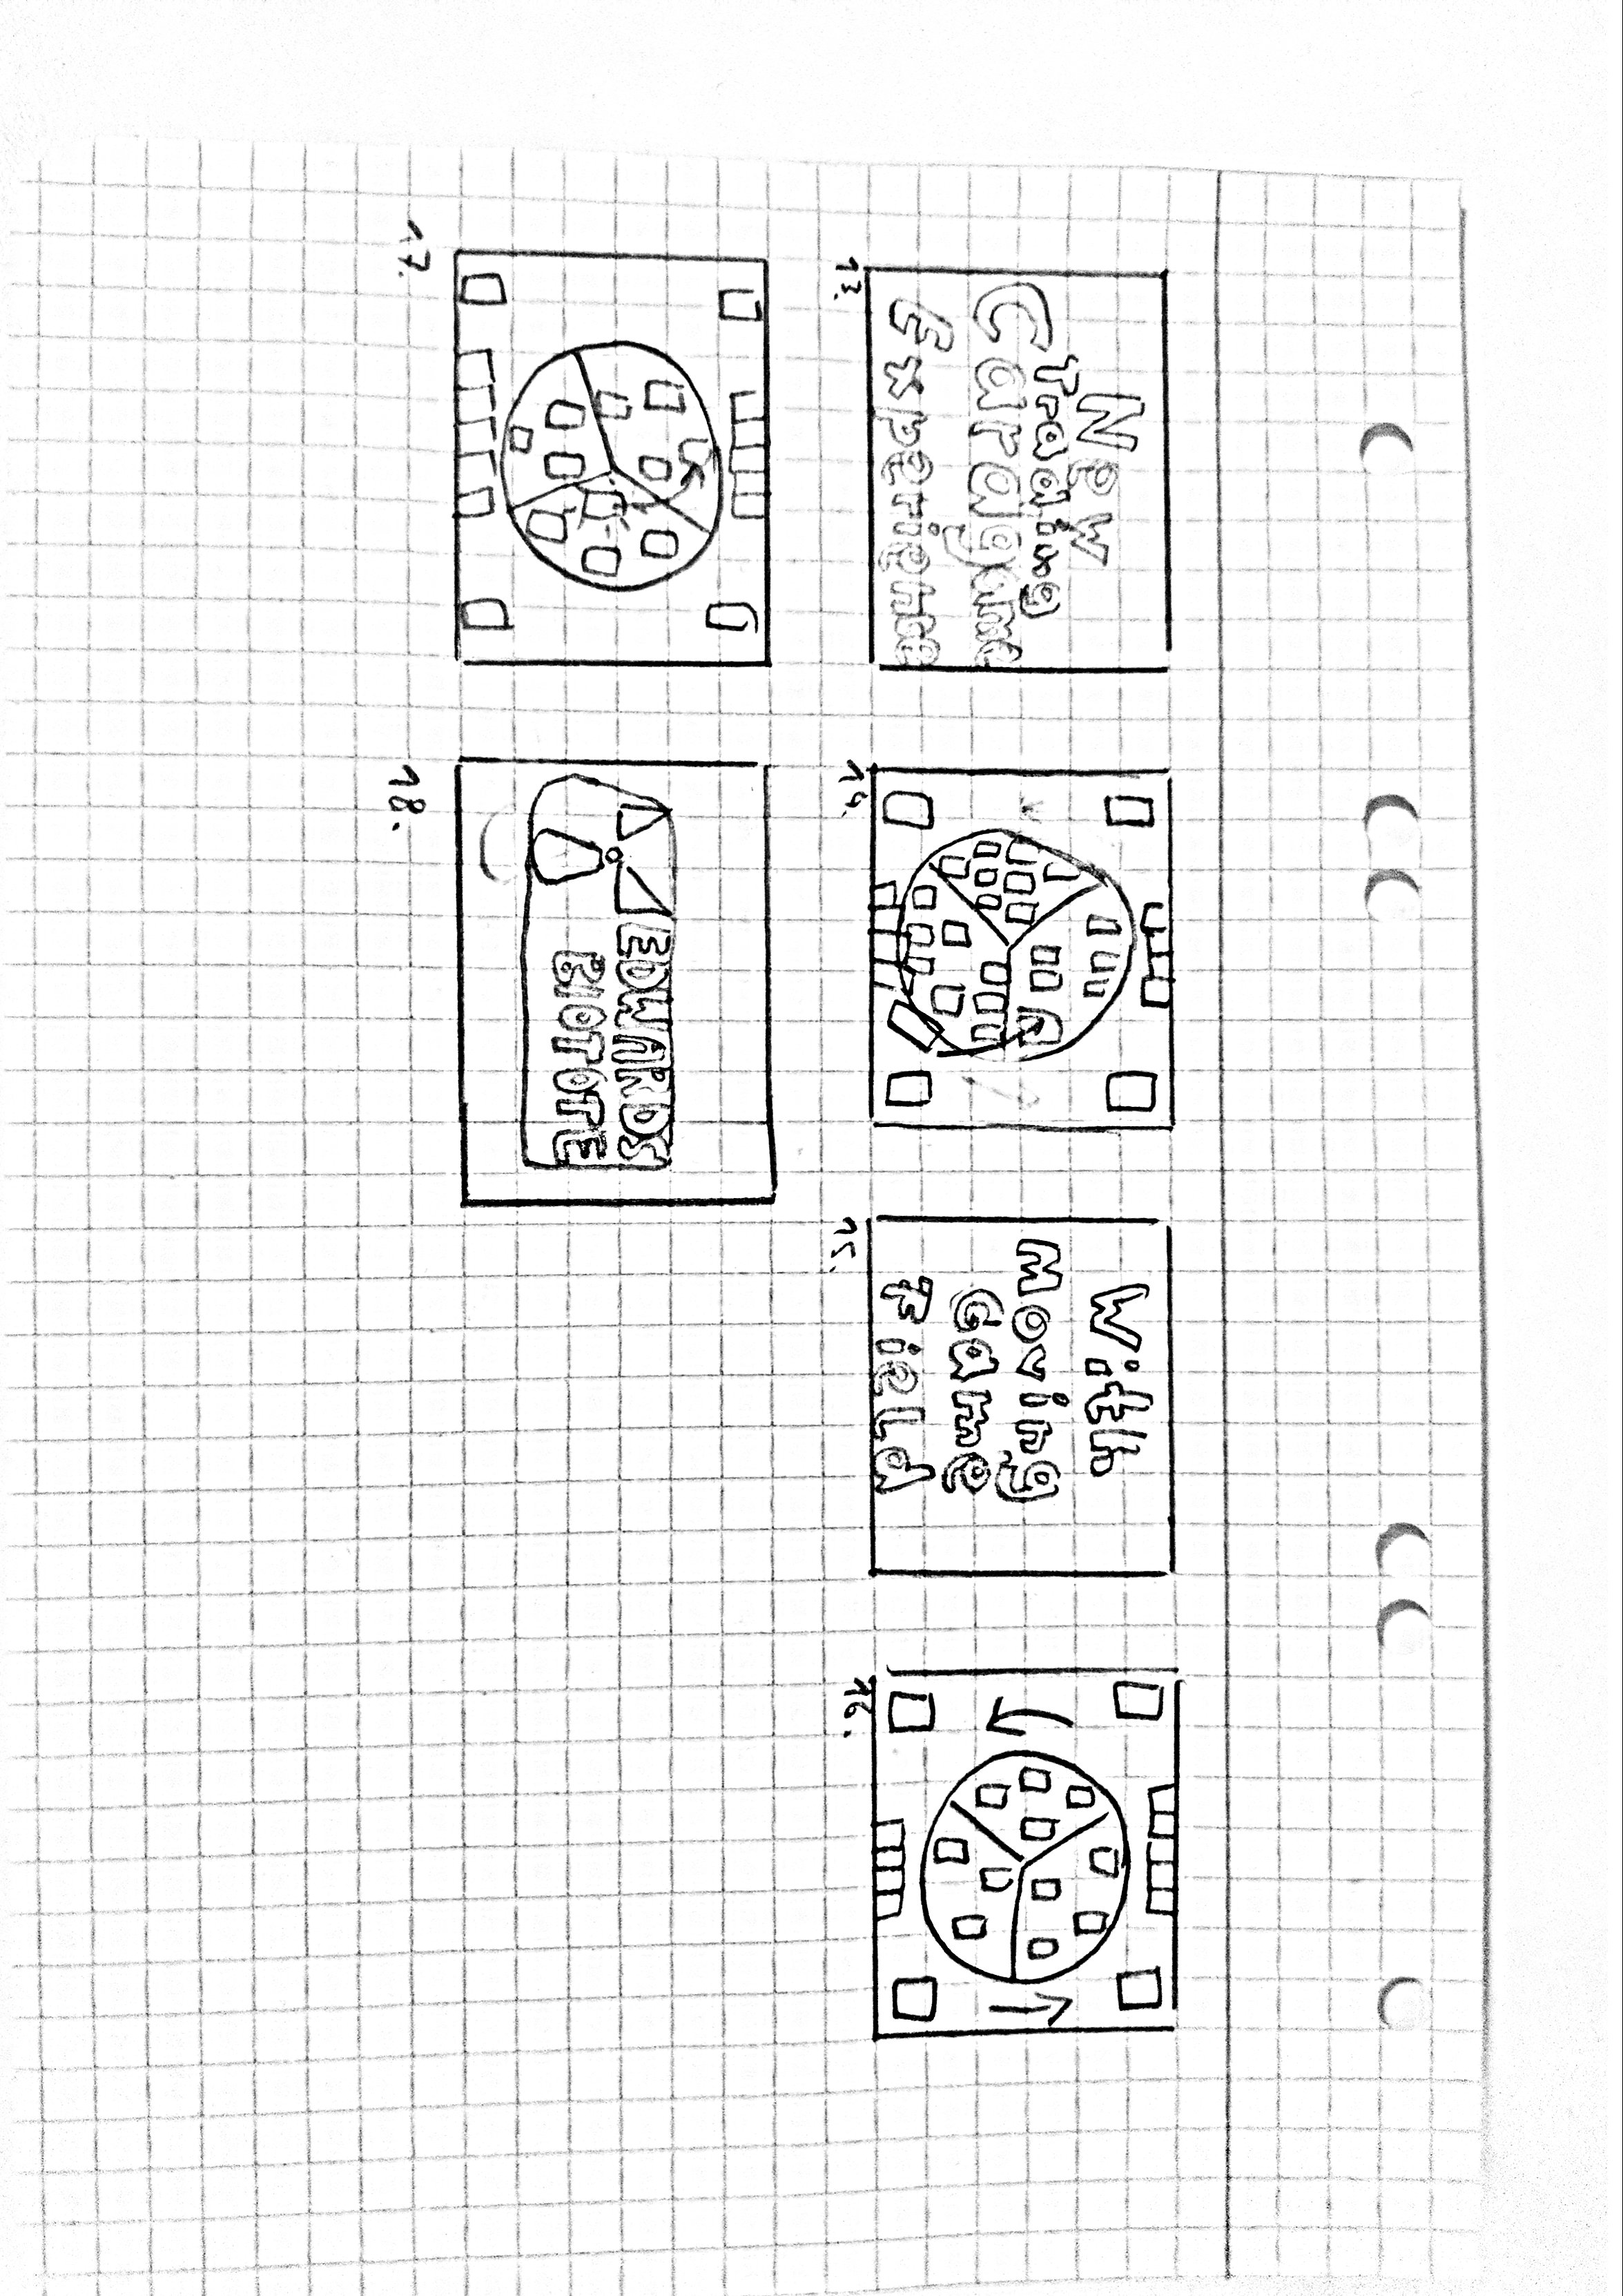
\includegraphics[width=4cm]{../img/storyboards/storyboard_3.JPG} }}
\caption{Storyboard: Spielfeld}%
 \label{fig:Storyboard: Spielfeld}%
\end{figure}

Nach einiger Überlegung wurde sich auf ein Storyboard geeinigt und den Trailer in 3 Abschnitte aufgeteilt, für die jeweils eine Person zuständig war. Abschnitt 1 ist die Vorgeschichte/Intro, Abschnitt 2 die Verwandlung der Kreaturen in mutierte Monster und Abschnitt 3 Ingame-Gameplay. Hier wird die Arbeit an Abschnitt 3 beschrieben.

In Abschnitt 3 soll das Gameplay des Spiels gezeigt werden und zwar so nah am Endprodukt wie möglich. Dies war nicht sehr leicht, weil manche Ideen zum Gameplay noch nicht absolut feststanden. Die Idee war es die Grundfunktionen des Gameplays zu zeigen wie z.B. Farbrad drehen, Strömungsrichtung, Zonenaktivierung und einen ausgeführten Angriff. In dieser weise könnte ein Spielzug eines Spielers aussehen und es war wichtig diesen Ablauf einzuhalten. Zum Animieren wurden hauptsächlich die original Spiele-Assets verwendet, wobei bei den Spezialeffekten und der Seitenleiste die Original-Buttons noch nicht feststanden.

\begin{figure}
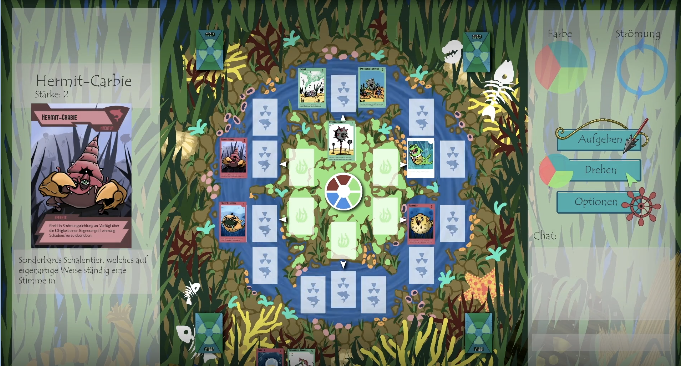
\includegraphics[width=0.8\textwidth]{../img/video_spielfeld.PNG}
\caption{Darstellung des Spielfelds im Trailer}
\label{fig:Videodarstellung Spielfeld}
\end{figure}

In Adobe After Effects wird anhand von Keyframes animiert. AE ist ein Compositing-Tool, das in Ebenen funktioniert, anders als Nuke(Compositing-Programm), das in Nodes aufgebaut wird.
Pro Ebene ist ein Asset eingefügt. Jedes Asset lässt sich beliebig drehen, vergrößern, transparent machen und bewegen. Diese ganzen Parameter lassen sich auch über Keyframes definieren. Keyframes sind von der Zeitleiste abhängig, d.h. an dem Zeitpunkt an dem ein Keyframe ist, müssen die eingestellten Parameter angewendet sein. Von einem Keyframe zum nächsten wird diese Änderung aber interpoliert dargestellt, wodurch eine gleichmäßige Änderung im Video zu sehen ist.

Dieser Workflow ist deutlich einfacher als Gameplay aufzunehmen oder vor allem Bild für Bild selber zu bearbeiten.

\subsubsection{Produktion Video Intro}
Für einen Einstieg in die Geschichtsthematik des Spieles wurde der Betrachter mittels einer Kamerafahrt über das Meer an den eigentlichen Veranstaltungsort mitgenommen.
Dafür wurde ein längliches Bild angefertigt, das in AfterEffects zu einer Komposition hinzugefügt wurde. Anschließend wurde eine neue “Kamera” erstellt und die 3D-Funktionen der Kompositionsebene aktiviert. Nun mussten nur noch zwei Keyframes gewählt werden, den Startkeyframe am unteren, sowie den Endkeyframe am oberen Ende des Bildes.
Da Wasser, noch spezifischer gesehen Wellenbewegungen, sehr komplex zu animieren sind, wurde für die nächste Szene eine Wellenreihe in Adobe Animate angefertigt. Das Programm ermöglichte es die “Meereszacken” durch Anfertigung und Abspielen verschiedenster Frames zum Rotieren zu bringen. In After Effects importiert ergaben diese hintereinander liegenden Reihen in unterschiedlicher Ablaufgeschwindigkeit die Illusion einer sich bewegenden Meeresoberfläche. 
Das angefertigte Schiff musste jetzt an die Bewegungen der vordersten Welle angepasst werden. Diese Bildverschiebung kann in After Effects durch das Verändern der Position als auch Rotation sowie durch das Setzen mehrerer Keyframes (siehe Abbildung x) visualisiert werden. Auch der Hintergrund sowie der Blitz musste vorerst angefertigt und implementiert werden. Um das Aufleuchten des Blitzes naturgetreuer darzustellen, wurde seine Darstellung zwischen Erscheinen und Verschwinden noch verdoppelt. 

\begin{figure}
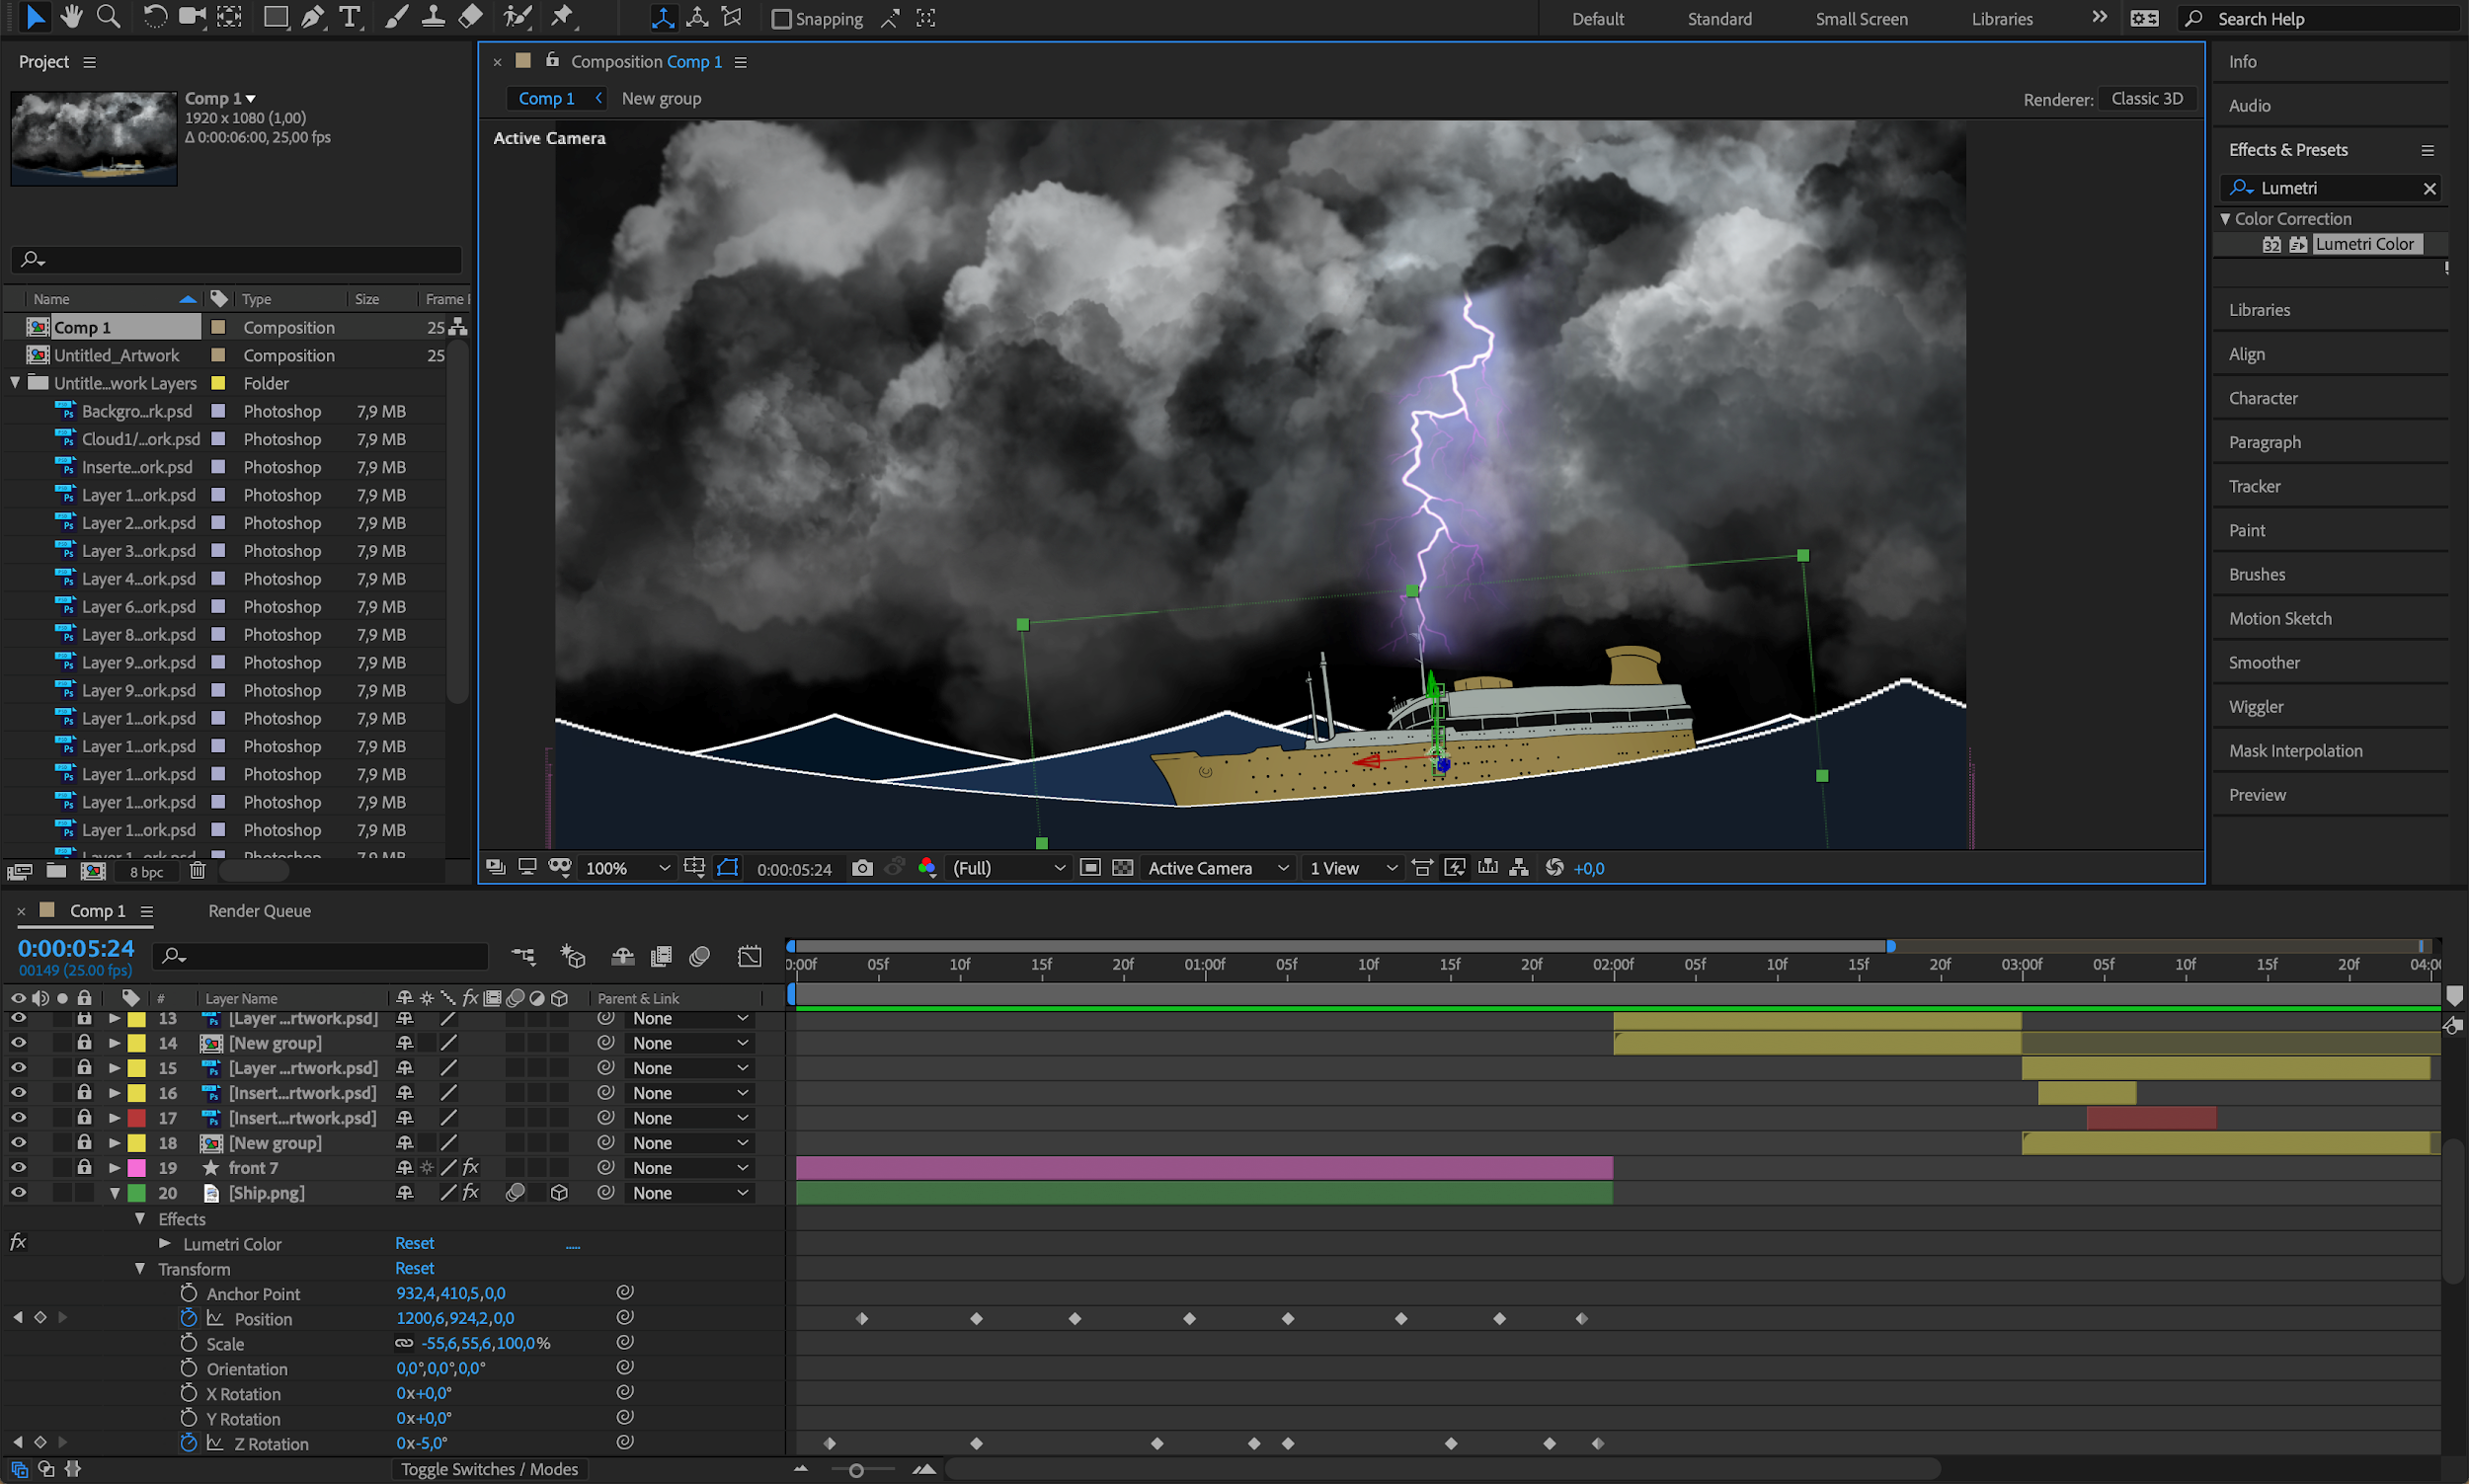
\includegraphics[width=0.5\textwidth]{../img/screenshot_aftereffects_intro.PNG}
\caption{Screenshot: After Effects Intro}
\label{fig:Screenshot: After Effects Intro}
\end{figure}